\documentclass[11pt,a4paper]{article}
\usepackage[utf8]{inputenc}
\usepackage{amsmath}
\usepackage{amsfonts}
\usepackage{graphicx}

\usepackage[table,xcdraw]{xcolor}

\usepackage{caption}
\usepackage{subcaption}
\usepackage{float} % para que floten las imagenes o algo asi...
\usepackage{wallpaper} %paquete para usar una imagen como encabezado!
\usepackage{hyperref} %para usar hypervinculos 
\usepackage[export]{adjustbox} %para usar marcos en imagenes
\usepackage{eurosym} % para el euro
\usepackage{transparent} %para las marcas de agua
\usepackage{eso-pic}  %para las marcas de agua
\definecolor{azul_marcos}{RGB}{0,128,159} %defino el color azul de los marcos
\usepackage{sectsty} %esto es para cambiar el color de las fuentes creo
\renewcommand{\familydefault}{\sfdefault} % cambiamos la fuente a una sans
\sectionfont{\color{azul_marcos}}  % sets colour of sections
\subsectionfont{\color{azul_marcos}}  % sets colour of sections
\usepackage{pdfpages} %para insertar pdfs
\usepackage{amssymb}
\usepackage{pstcol} % para color
\usepackage{pst-node} % para diagramas
\usepackage{pst-plot} % para representacion de dat
\usepackage[spanish]{babel}
\addto\captionsspanish{\renewcommand\chaptername{Bloque}}
%\usepackage[total={18cm,21cm},top=2cm, left=2cm]{geometry}
\usepackage{anysize}
\pagestyle{plain}
%\markboth{left head}{right head}
%\markright{Guía de impresión FlexiSMART}
\marginsize{3cm}{2cm}{2.5cm}{1cm}
\title{FlexiSMART Druckanweisungen}
\date{}

%configuracion de la marca de agua
\AddToShipoutPicture{
    \put(0,0){
        \parbox[b][\paperheight]{\paperwidth}{%
            \vfill
            \centering
            {\transparent{0.2}
\includegraphics[scale=1.25]{FOTOS/logofff}}%
            \vfill
        }
    }
}

\begin{document}
\ULCornerWallPaper{1}{FOTOS/header}
\LLCornerWallPaper{1}{FOTOS/footer}
%\maketitle
%\tableofcontents

\includepdf{PDF/DE_PORTADA.pdf}
\section{Was ist FlexiSMART?}FlexiSMART ist ein Filament für 3D FFF/FDM-Druck aus thermoplastischen elastomeren Polymeren (TPE) mit chemischen Zusätzen um es einfacher zum Drucken für die meisten 3D-Drucker auf dem Markt zu machen.
\\\\
FlexiSMART ist flexibel und behält seine Form wenn es gefaltet, verdreht oder gedehnt wird.

\section{Weshalb FlexiSMART verwenden?}
FlexiSMART eröffnet Ihnen eine neue Welt an Möglichkeiten dank der flexiblen Natur seiner Filamente. Von nun an können Sie Objekte druck, die Sie zuvor mit starren Filamenten nicht drucken konnten: Hüllen für Smartphones, Tablets, Slippers, Schablonen, RC-Räder, Prothesen, Silent Blocks, Zahnräder, die gewissen Anpassungsfähigkeiten benötigen und generell jedes Objekt, das Sie sich vorstellen können und für welches Sie einen Nutzen finden.
\\\\
FlexiSMART wurde designt um einfach druckbar zu sein:
\begin{itemize}
\item Es hat eine gewisse Starrheit, so dass es von den moisten direkten Extrudern ohne oder mit nur wenigen Anpassungen gedruckt werden kann.
\item Die Anhaftung ist ausgezeichnet. Sie können es ohne heißes Bett drucken.
\item Der Widerstand ist sehr hoch, weshalb de gedruckten Stücke nicht so schnell verwittern.
\item Es sind die flexiblen Filamente mit dem attraktivsten Preis in Europa. 
\end{itemize}

\section{Datenblatt und Druckparameter}

\begin{table}[H]
\centering
\caption*{Datenblatt}
\begin{tabular}{|
>{\columncolor[HTML]{FFFFFF}}l |
>{\columncolor[HTML]{FFFFFF}}c |}
\hline
\multicolumn{1}{|c|}{\cellcolor[HTML]{FFFFFF}\textbf{Material}}   & FlexiSMART (TPE)   \\ \hline
\textbf{Verfügbare Farben}              & 11                 \\ \hline
\textbf{Verfügbare Formate}             & 1kg, 250gr         \\ \hline
\textbf{Thermische Deflexionstemperatur} & 90ºC               \\ \hline
\textbf{Fusionstemperatur}            & 160ºC              \\ \hline
\textbf{Dekompositionstemperatur}    & \textgreater 240ºC \\ \hline
\textbf{Dichte}                         & 0.96 gr / cm3      \\ \hline
\textbf{Maximale Dehnbarkeit}              & 600\%              \\ \hline
\end{tabular}
\end{table}
\begin{table}[H]
\centering
\caption*{Druckparameter empfohlen bei einer 0.4 mm Düse}
\begin{tabular}{|
>{\columncolor[HTML]{FFFFFF}}l |
>{\columncolor[HTML]{FFFFFF}}c |}
\hline
\multicolumn{1}{|c|}{\cellcolor[HTML]{FFFFFF}\textbf{Empfohlene Drucktemperatur}} & 195º-220º              \\ \hline
\textbf{Empfohlene Druckgeschwindigkeit}                         & 20-60mm/s              \\ \hline
\textbf{Temperatur des heißen Bettes}                                  & \textgreater 18º (benötigt kein heißes Bett)        \\ \hline
\textbf{Optimale Schichthöhe}                                      & 0.2 mm                 \\ \hline
\textbf{Perimeter}                                                 & 3                      \\ \hline
\textbf{Oberste, solide Schicht}                                           & 5                      \\ \hline
\textbf{Rückzug}                                                 & Deaktiviert oder reduziert \\ \hline
\end{tabular}
\end{table}

Sie können unser volles Druckprofil von den Hauptlaminierungsprogrammen (Cura, Slic3r und SImplify3D) von unserer Webseite herunterladen:
\\\\
\centerline{ {\huge \url{www.fffworld.com/documentation} } }
\\\\
Optimale Parameter sind abhängig vom 3D-Drucker, den Sie verwenden, jedoch sind es gute Parameter zur Abschätzung. Mit ein paar Drucken werden Sie in der Lage sein die Grenzen und die besten Einstellungen für Ihre Maschine zu finden.
\section{Probleme und Lösungen}
	\subsection{Probleme beim Extrudieren von FlexiSMART}
Die größte Herausforderung beim Drucken mit FlexiSMART und anderen flexiblen Fäden ergibt sich aus der Natur des Materials selbst, durch die Flexibilität kann es nicht so leicht geschoben werden wie starre Materialien, in gleicher Weise wie man ein Seil nicht drücken kann.
\\\\
Das Problem entsteht, wenn es Lücken auf bestimmten Teilen des Extruders gibt, insbesondere zwischen dem Drive-Gear (das gezahnte Rad, das den Faden drückt) und dem Loch, durch das der Faden das Hot-End erreicht(metallischer Punkt, der den Faden schmilzt).
\\\\
Wenn dieser Raum zu groß ist, tendiert das Filament dazu aus seiner Straße auszubrechen und einen Knoten zu erzeugen, der durch eine Seite des Extruders stößt, wie auf dem Bild zu sehen ist.
\begin{figure}[H]
\centering
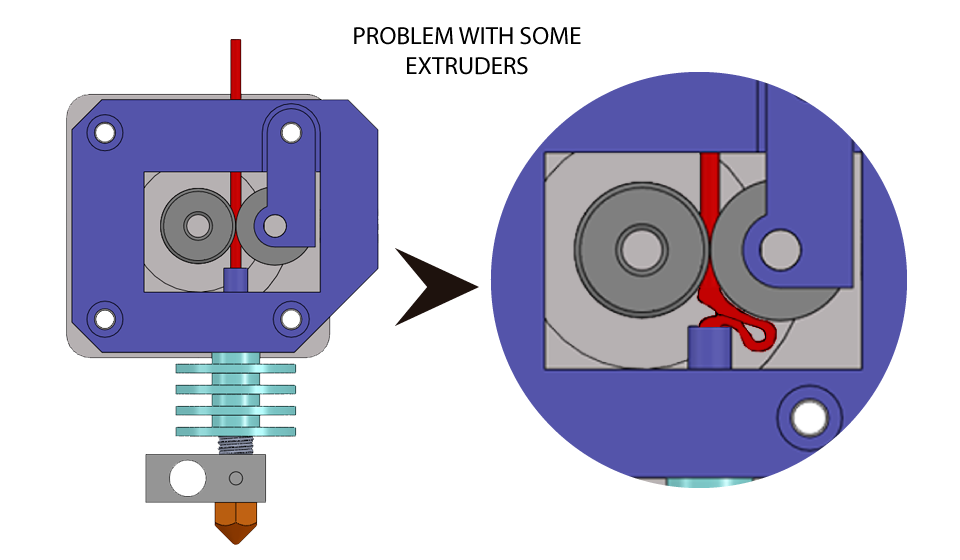
\includegraphics[width=0.5\textwidth,cfbox=azul_marcos 4pt 0pt]{FOTOS/NUDOS1}
\caption*{NON-optimized extruder for printing flexible filaments}
\end{figure}
Dieses Problem ist größer, wenn Sie die 1,75 mm-Filamente benutzen, da es unter Verwendung von zu geringem Sog eher zum Ausbrechen tendiert.
\\\\
Die Extrusionsgeschwindigkeit ist bestimmend für das Auftreten dieses Problems. Wenn der Extruder versucht, den Faden mit der maximalen Geschwindigkeit zu schieben, wird ein Aufwärtsdruck erzeugt, der den Faden von seinem Weg abbringt. Deshalb ist die allgemeine Empfehlung den Druck in einer langsamen oder sehr langsamen Geschwindigkeit zu starten und dann zu erhöhen, bis Sie die maximale Geschwindigkeit Ihres Extruders erreichen. Die Größe der Düse wirkt sich auch auf die maximale Grenzgeschwindigkeit aus, denn je größer diese ist, desto mehr geschmolzenes Material kann pro Zeiteinheit extrudiert werden und daher wird die Geschwindigkeit, mit der es durchgeführt werden kann, erhöht.
\\\\
Die Extruder, welche entwickelt wurden um flexible Filamente zu nutzen, minimieren die Lücken und verhindern so, dass das Filament einen Tropfen bildet und heraussteht und sie enthalten ein System mit doppeltem Drive-Gear um das Filament mit Präzision zu kanalisieren und das genannte Problem vollständig zu umgehen während sie gleichzeitig eine höhere Druckgeschwindigkeit ermöglichen.
\begin{figure}[H]
\centering
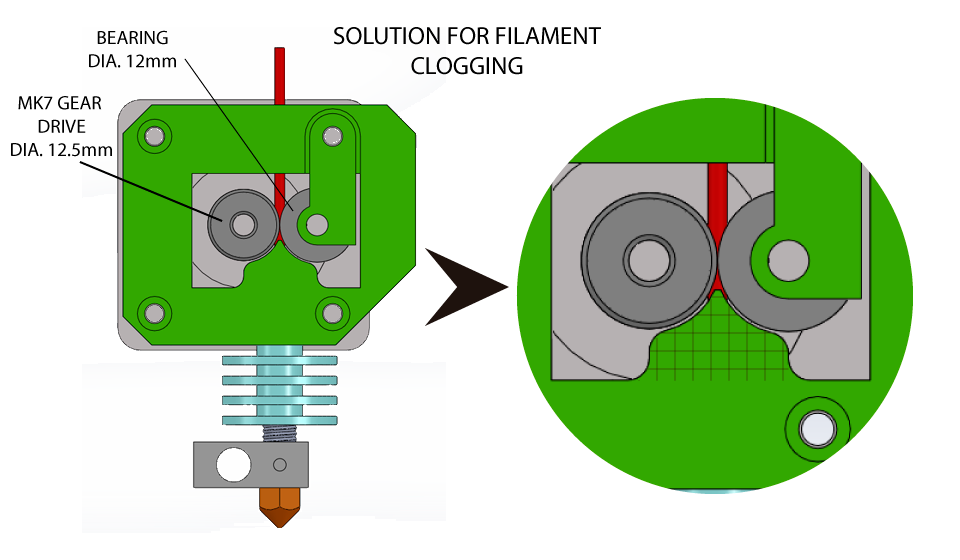
\includegraphics[width=0.5\textwidth,cfbox=azul_marcos 4pt 0pt]{FOTOS/NUDOS2}
\caption*{Optimized extruder for printing flexible filaments}
\end{figure}
\emph{FlexiSMART wurde mit diesen Problemen im Hinterkopf designt und hat eine Steifigkeit, welche andere flexible Filamente überragt und hilft diese zu reduzieren.}
\\\\
Diese Probleme könnten jedoch auf Extrudern auftreten, die nicht für elastische Materialien ausgelegt sind.
	\subsection{Vorbereitung des Extruders um FlexiSMART zu drucken}Wenn Sie eines der bereits erwähnten Probleme haben, müssen Sie wahrscheinlich Ihren Extruder anpassen oder ersetzen. In diesem Sinne gibt es einige Optionen, die wir weiter unten detaillierter erläutern.
		\subsubsection{Modifizieren Ihres Extruders}
Manchmal ist es möglich FlexiSMART auf nicht optimierten Extrudern zu benutzen, indem man einige Änderungen am Extruder selbst vornimmt.
\\\\
Wenn Sie Probleme haben FlexiSMART zu drucken, schlagen wir vor, dass Sie die folgenden Ratschläge befolgen, in der Reihenfolge aufsteigender Komplexität.
			\paragraph{Die Vorgehensweise, durch die das Filament an das heiße Ende gelangt}\mbox{}\\\\
Wenn Sie einen Extruder mit einem Kunststoffkörper verwenden, wie dies bei bedruckbaren Extrudern der Fall ist, empfehlen wir Ihnen das Folgende zu versuchen.
\\\\
Ordnen Sie leicht die Ränder des Lochs genau unter dem Drive-Hear, dem Loch durch welches der Faden an das Hot-End geleitet wird. Auf diese Weise können Sie die Reibung und Pannen vermeiden, die die zuvor beschriebenen Knoten provozieren können. 
\\\\
Es könnte notwendig sein einen Teil des Extruders abzunehmen um diesen Operation durchführen zu können.
			\paragraph{Führen Sie die Teflonröhre in den Extruder ein}\mbox{}\\\\
Eine zweite Möglichkeit, kompliziertere aber effektiver, ist es ein Teflonrohr (PTFE) in das erwähnte Loch einzuführen. Diese Technik ermöglicht es auch, den Raum mit dem Drive-Gear zu reduzieren, da die Röhre nahe an jenes platziert werden kann. Sie können sogar den Eintritt in die Teflonröhre ändern, um es der Form des Drive-Gear anzupassen, was nur noch minimal Platz übrig lässt.
\\\\
Im allgemeinen beinhaltet diese Technik das Aufbohren des Extruders um das Einführen des genannten Teflonschlauches zu ermöglichen. Hier sehen Sie einige Bilder des Ergebnisses:
\begin{figure}[H]
    \centering
    \begin{subfigure}[b]{0.3\textwidth}
        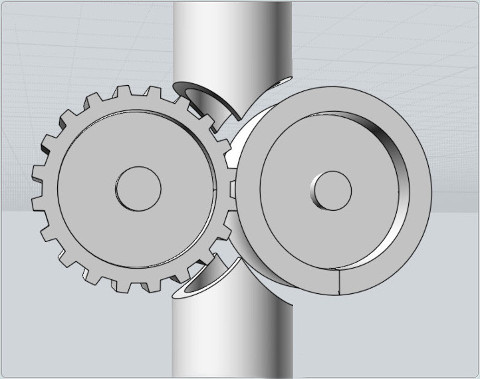
\includegraphics[width=\textwidth,cfbox=azul_marcos 4pt 0pt]{FOTOS/TEFLON1}
    \end{subfigure}
    ~ %add desired spacing between images, e. g. ~, \quad, \qquad, \hfill etc. 
      %(or a blank line to force the subfigure onto a new line)
    \begin{subfigure}[b]{0.3\textwidth}
        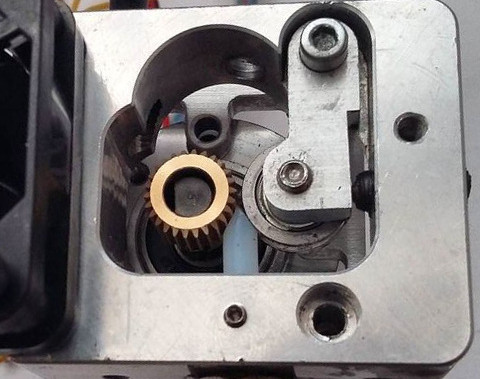
\includegraphics[width=\textwidth,cfbox=azul_marcos 4pt 0pt]{FOTOS/TEFLON2}
    \end{subfigure}
    ~ %add desired spacing between images, e. g. ~, \quad, \qquad, \hfill etc. 
    %(or a blank line to force the subfigure onto a new line)
    \begin{subfigure}[b]{0.3\textwidth}
        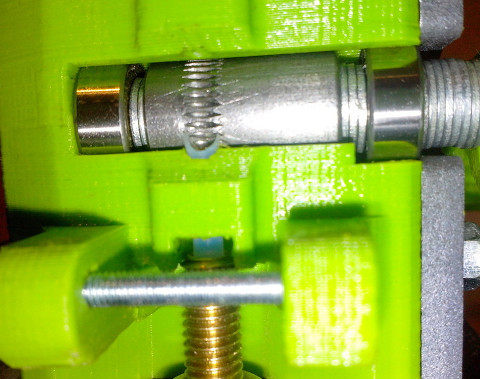
\includegraphics[width=\textwidth,cfbox=azul_marcos 4pt 0pt]{FOTOS/TEFLON3}
    \end{subfigure}
    \caption*{PTFE (Teflon) tube insertions}
\end{figure}
			\paragraph{Drucken Sie eine Führung für das Filament und legen Sie in den Extruder}\mbox{}\\\\
Die dritte Möglichkeit ist es, ein Stück auszudrucken, dass für das Filament als Leitfaden fungiert und es unter das Drive-Gear zu legen. Diese Stücke haben in der Regel eine dreieckige Form und sollten unter Beachtung der Abmessung jedes Extruders entworfen werden.
\\\\
Im Internet auf Websites wie \url{www.thingiverse.com}, können Sie diese Art von Adaptern für einige der üblichen Extruder herunterladen. Dies ist jedoch ein einfaches Design, welches Personen mit Kenntnissen im 3D-Druck einfach von Grund auf selbst erstellen können.
\begin{figure}[H]
    \centering
    \begin{subfigure}[b]{0.5\textwidth}
        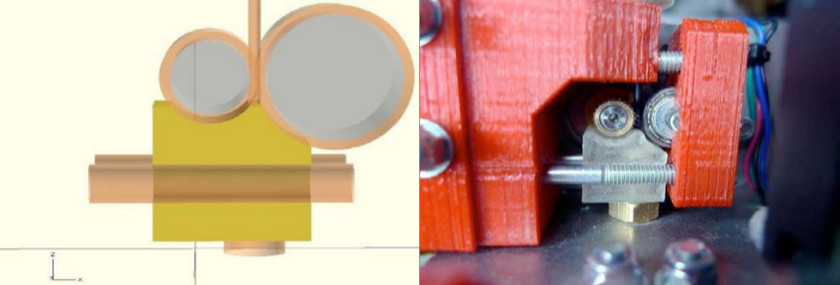
\includegraphics[width=\textwidth,cfbox=azul_marcos 4pt 0pt]{FOTOS/GUIA1}
    \end{subfigure}
    ~ %add desired spacing between images, e. g. ~, \quad, \qquad, \hfill etc. 
      %(or a blank line to force the subfigure onto a new line)
    \begin{subfigure}[b]{0.5\textwidth}
        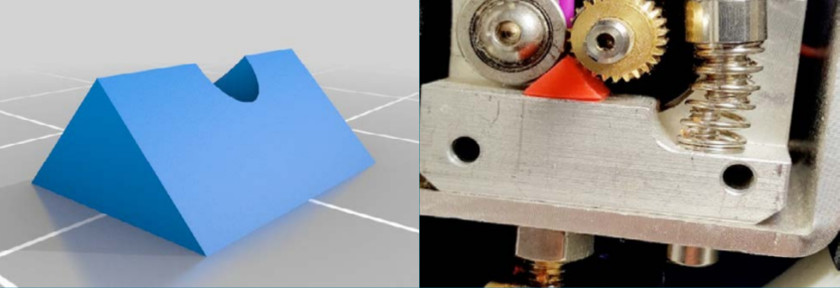
\includegraphics[width=\textwidth,cfbox=azul_marcos 4pt 0pt]{FOTOS/GUIA2}
    \end{subfigure}
    ~ %add desired spacing between images, e. g. ~, \quad, \qquad, \hfill etc. 
    %(or a blank line to force the subfigure onto a new line)
    \begin{subfigure}[b]{0.5\textwidth}
        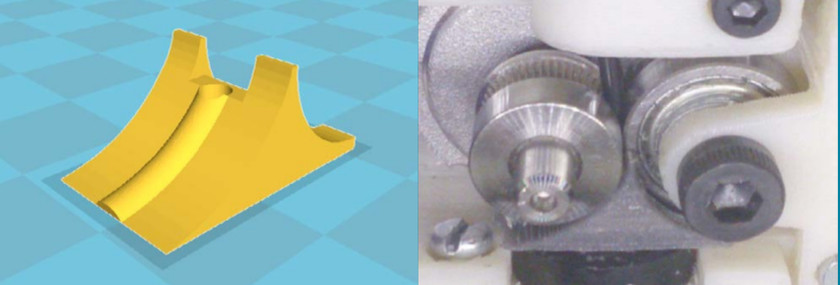
\includegraphics[width=\textwidth,cfbox=azul_marcos 4pt 0pt]{FOTOS/GUIA3}
    \end{subfigure}
    \caption*{Printable filament guides}
\end{figure}	

	\paragraph{Einstellen vom Druck des Drive-Gears über das Filament}\mbox{}\\\\
Da dies ein flexibles Material ist, ist es besonders wichtig, dass der Druck des Mechanismus, der das Filament in Richtung des Hot-End schiebt, nicht übermäßig hoch ist. Ein Überschuss an Druck kann in den steifen Filamenten kleine Einkerbungen in der Oberfläche erzeugen, aber im Fall von FlexiSMART würde übermäßiger Druck den Abschnitt des Filaments verunstalten und ihm eine ovale Form geben, die den Extruder anfälliger für Verstopfungen macht.
\\\\
Die Extruder, welche für das Drucken von flexbiblen Filamenten entwickelt wurden, berücksichtigen dies und haben einen Mechanismus um den Druck des Zugmechanismus zu regulieren. Wenn Ihr Extruder die Regulierung eines solchen Drucks erlaubt, empfehlen wir, dass Sie ihn anpassen, wenn Sie FlexiSMART verwenden. Der adequate Druck ist das erforderliche Minimum, dass der Extruder benötigt um den Faden zu bewegen.
\\\\
Wenn Ihr Extruder diesen Mechanismus nicht hat, können Sie den Druck dennoch reduzieren, indem Sie die Feder austauschen oder die mögliche Route durch einen Keil am richtigen Ort reduzieren. Als Beispiel zeigen wir ein Bild, wie man den Druck in einem Extruder reduzieren kann, der nicht bereit dafür ist:
\begin{figure}[H]
\centering
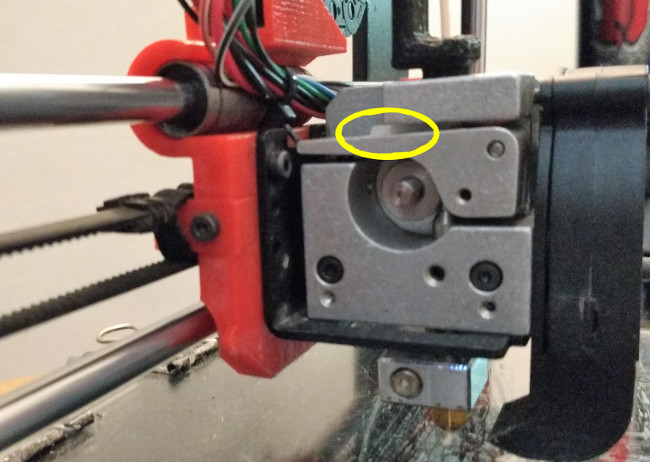
\includegraphics[width=0.5\textwidth,cfbox=azul_marcos 4pt 0pt]{FOTOS/SOLUCION1}
\caption*{HeatCore Extruder. BQ Hephestos and BQ Witbox}
\end{figure}
			\paragraph{Hinzufügen von Spannungen zwischen der Rolle und dem Extruder}\mbox{}\\\\
Es wurde gezeigt, dass es in einigen Druckermodellen praktisch ist, dass es bei der Verwendung von flexiblen Faden eine gewisse Spannung zwischen der Trommel und dem Extruder in einer Weise gibt, dass der Faden nicht hängen bleibt.
\\\\
Um dies zu erhalten, können Sie versuchen die Rolle zu stoppen, so dass der Extruder leicht vom Faden ziehen muss um es zu entwirren. Sie können auch ein ähnliches Zubehör platzieren wie auf dem Foto, um das gleiche Ziel zu erreichen.
\begin{figure}[H]
\centering
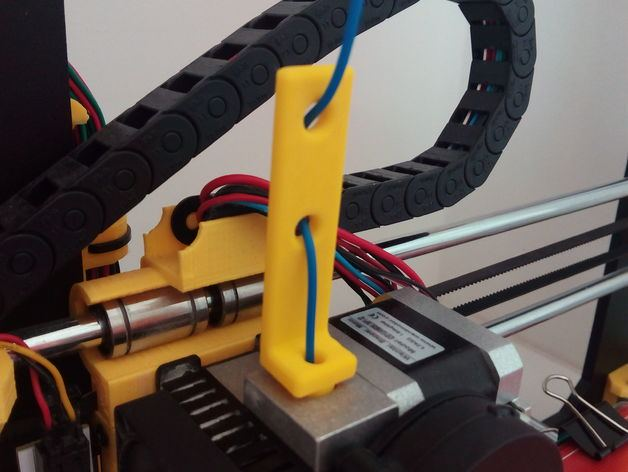
\includegraphics[width=0.5\textwidth,cfbox=azul_marcos 4pt 0pt]{FOTOS/SOLUCION2}
\caption*{Designed for BQ Unibody and BQ Hephestos extruder}
\end{figure}
		\subsubsection{Ersetzen Sie Ihren Extruder mit einem optionalen}
Heutzutage sind flexible Filamente bis zu dem Punkt beliebt geworden, wo es schwierig für Drucker der letzten Generation ist, sie zum Drucken vorbereitet.
\\\\
Außerdem haben viele Designer bedruckbare Extruder designt, die mit FlexiSMART und anderen Filamenten arbeiten können. Diese Extruder können von Seiten wie Thingiverse heruntergeladen und zu Hause ausgedruckt und zusammengebaut werden.
\\\\
Die kommerziellen Extruder sind auch jedes Mal besser vorbereitet um flexible Filamente zu drucken, die erworben werden und auf unsere Drucker montiert werden können.
			\paragraph{DIY bedruckbare Extruder}
\mbox{}\\\\
Einige dieser Extruder sind von Grund auf neu entwickelt und andere sind gegenüber bestehenden Designs modifiziert. Hier präsentieren wir eine unvollständige Liste von Extruderdesigns, die aus dem Internet heruntergeladen werden können. Wenn Sie den Links folgen, können Sie die vollständige Liste der Komponenten sowie die Montageanleitung und Kommentare anderer User finden.
\\\\
Das Hot-End, dass auf dem Extruder installiert wird, muss innen ein Teflonstück (PTFE) haben um Reibung zu vermeiden, damit das FlexiSMART korrekt geschoben wird. FlexiSMART wurde auf den folgenden Hot-Ends erfolgreich getestet\footnote{Sie müssen bedenken, dass besagte Tests mit Original Hot-Ends gemacht wurden und wir das Ergebnis auf Nachahmungen dieser nicht garantiert werden kann.}:
\begin{itemize}
\item J-Head MKV-B
\item Budassnozzle V1.3
\item E3D v6
\item Leonnozzle V2
\end{itemize}
Je nachdem welche Drucker Sie verwenden, werden einige dieser Extruder leichter zu installieren sein unter der Vorraussetzung, dass sie den ursprünglichen Extruder der Maschine ersetzen könnten.
\begin{figure}[H]
    \centering
    \begin{subfigure}[b]{0.4\textwidth}
        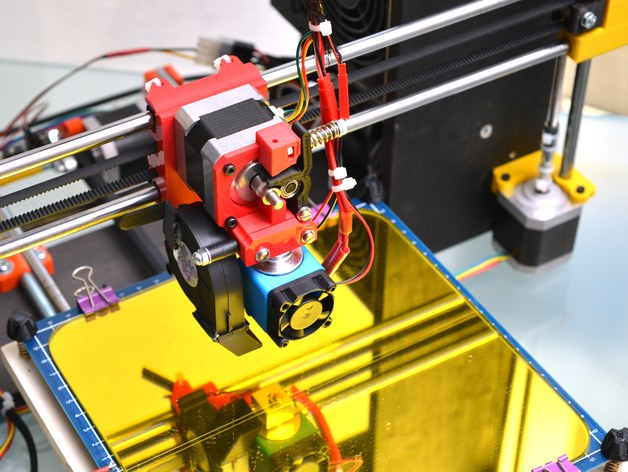
\includegraphics[width=\textwidth,cfbox=azul_marcos 4pt 0pt]{FOTOS/EXTRUSOR1}
		\caption*{\href{http://www.thingiverse.com/thing:147705}{{\footnotesize Direct-drive hinged extruder for E3D/J-Head hot-end (Prusa i3) by ffleury}}}
    \end{subfigure}
    ~ \qquad%add desired spacing between images, e. g. ~, \quad, \qquad, \hfill etc. 
      %(or a blank line to force the subfigure onto a new line)
    \begin{subfigure}[b]{0.4\textwidth}
        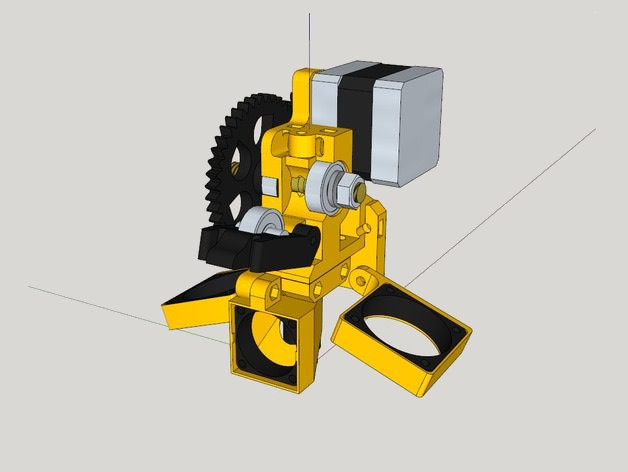
\includegraphics[width=\textwidth,cfbox=azul_marcos 4pt 0pt]{FOTOS/EXTRUSOR2}
		\caption*{\href{http://www.thingiverse.com/thing:512338}{{\footnotesize Wade L3K Extruder (prusa I3) compatible filament flexible By Skarab}}}
    \end{subfigure}
\end{figure}
\begin{figure}[H]
    \centering
    ~ %add desired spacing between images, e. g. ~, \quad, \qquad, \hfill etc. 
    %(or a blank line to force the subfigure onto a new line)
    \begin{subfigure}[b]{0.4\textwidth}
        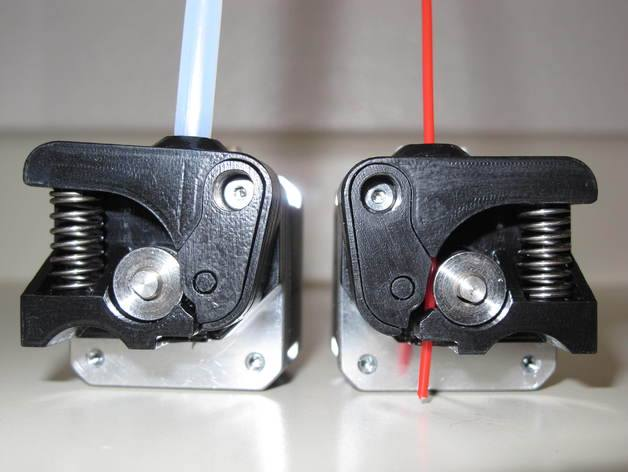
\includegraphics[width=\textwidth,cfbox=azul_marcos 4pt 0pt]{FOTOS/EXTRUSOR3}
		\caption*{\href{http://www.thingiverse.com/thing:403438}{{\footnotesize Printrbot Flexible Filament Direct Drive Extruder by thirdhorizon}}}
    \end{subfigure}
    ~ \qquad %add desired spacing between images, e. g. ~, \quad, \qquad, \hfill etc. 
    %(or a blank line to force the subfigure onto a new line)
    \begin{subfigure}[b]{0.4\textwidth}
        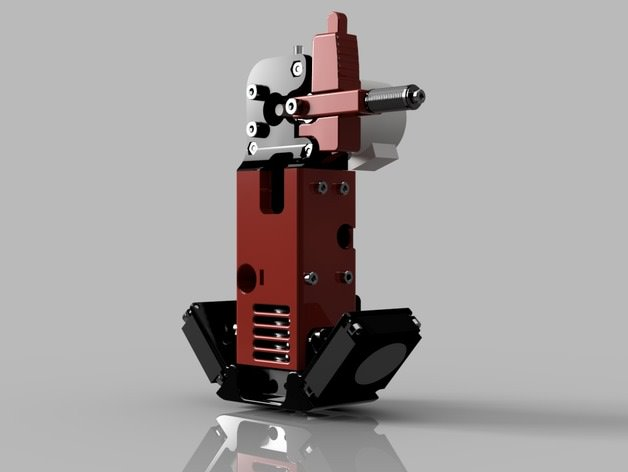
\includegraphics[width=\textwidth,cfbox=azul_marcos 4pt 0pt]{FOTOS/EXTRUSOR4}
		\caption*{\href{http://www.thingiverse.com/thing:1102900}{{\footnotesize Ultimaker 2 PG35L Direct Drive Extruder for 1.75mm E3D v6 Hotend by jasonatepaint}}}
    \end{subfigure}
\end{figure}
			\paragraph{Kommerzielle Extruder}\mbox{}\\\\
Der Erwerb eines kommerziellen Extruders ist teurer als ein zu Hause selbstgebauter, hat jedoch in der Regel eine bessere Leistung als dieser und ist die beste Wahl, wenn Sie vorhaben intensiv flexible Filamente zu verwenden.
\\\\
Diese Extruder wurden speziell entwickelt um die Probleme aller zuvor genannten Nachteile zu vermeiden und einige können FlexSMART bei Geschwindigkeiten höher als 70 mm/s nicht extrudieren.
\begin{figure}[H]
    \centering
    \begin{subfigure}[b]{0.4\textwidth}
        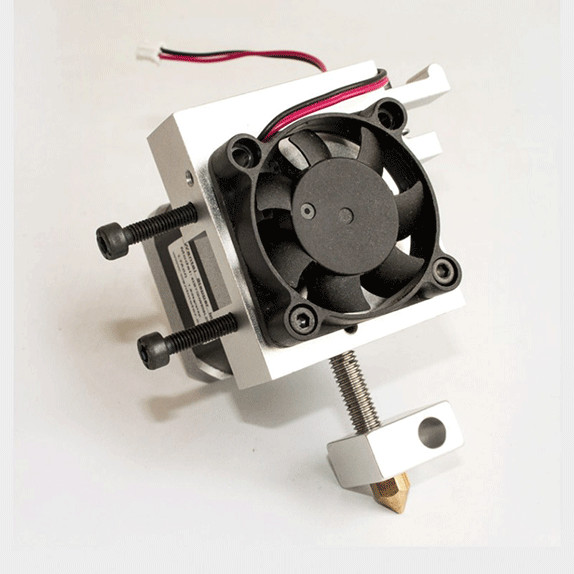
\includegraphics[width=\textwidth,cfbox=azul_marcos 4pt 0pt]{FOTOS/EXTRUSOR5}
		\caption*{\href{http://www.recreus.com}{{\footnotesize Recreus Extruder - Price aprox. 100\euro}}}
    \end{subfigure}
    ~ \qquad%add desired spacing between images, e. g. ~, \quad, \qquad, \hfill etc. 
      %(or a blank line to force the subfigure onto a new line)
    \begin{subfigure}[b]{0.4\textwidth}
        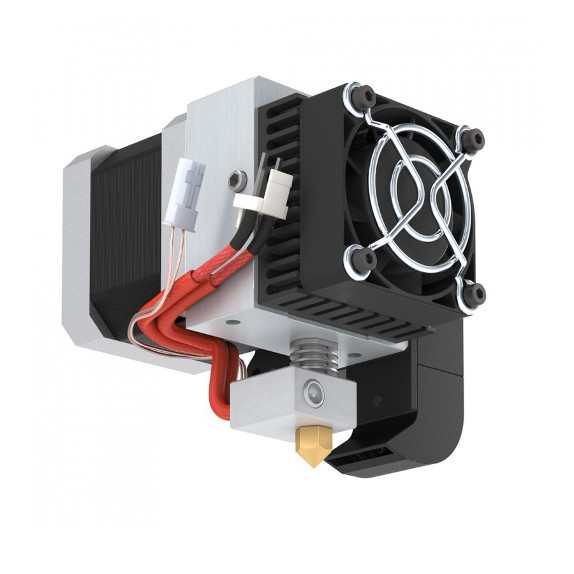
\includegraphics[width=\textwidth,cfbox=azul_marcos 4pt 0pt]{FOTOS/EXTRUSOR6}
		\caption*{\href{http://www.bq.es}{{\footnotesize BQ HeatCore DDG Extruder - Price 140\euro}}}
    \end{subfigure}
\end{figure}
\begin{figure}[H]
    \centering
    ~ %add desired spacing between images, e. g. ~, \quad, \qquad, \hfill etc. 
    %(or a blank line to force the subfigure onto a new line)
    \begin{subfigure}[b]{0.4\textwidth}
        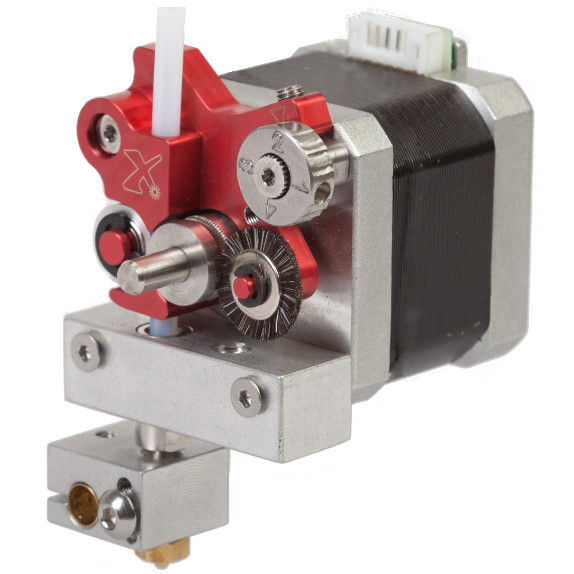
\includegraphics[width=\textwidth,cfbox=azul_marcos 4pt 0pt]{FOTOS/EXTRUSOR7}
		\caption*{\href{https://flexionextruder.com/}{{\footnotesize Flexion Extruder - Price aprox. 140\euro}}}
    \end{subfigure}
    ~ \qquad %add desired spacing between images, e. g. ~, \quad, \qquad, \hfill etc. 
    %(or a blank line to force the subfigure onto a new line)
    \begin{subfigure}[b]{0.4\textwidth}
        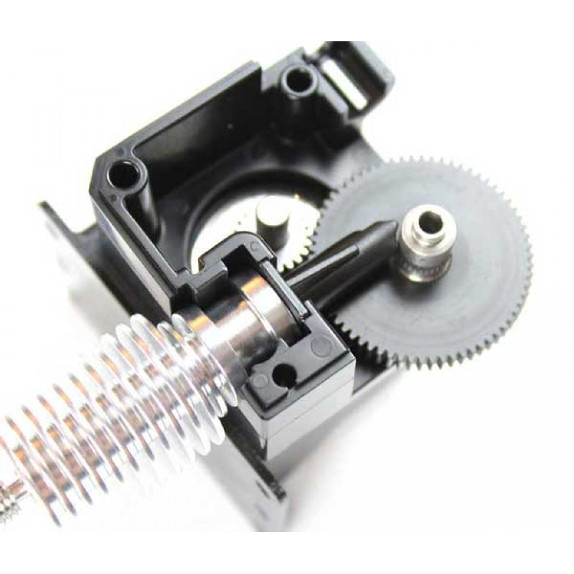
\includegraphics[width=\textwidth,cfbox=azul_marcos 4pt 0pt]{FOTOS/EXTRUSOR8}
		\caption*{\href{www.e3d-online.com}{{\footnotesize Titan Extruder - Price aprox. 70\euro}}}
    \end{subfigure}
\end{figure}
\section{Rat für eine optimale Nutzung von FlexiSMART}
	\subsection{Rückzug}
Rückzug ist eine verwendete Technik von 3D-FFF/FDM-Druckern um die Fertigstellung der Stücke zu verbessern. Es besteht aus Befehlen an den Extruder ein paar Zentimeter Faden zurückzuziehen wenn er die Position ändert, um die Bespannung oder das Auftreten von kleinen Fäden des Filaments auf verschiedene Teile des Druckstückes im Druck zu vermeiden.
\begin{figure}[H]
\centering
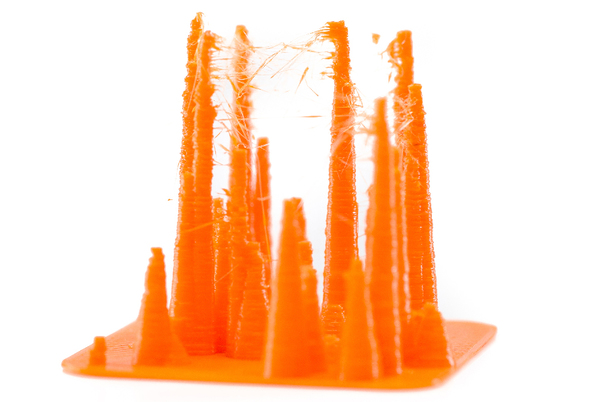
\includegraphics[width=0.5\textwidth,cfbox=azul_marcos 4pt 0pt]{FOTOS/RETRACCION1}
\caption*{A part with stringing problems}
\end{figure}
Wenn flexible Fäden verwendet werden, kann es passieren, dass durch den Versuch eines sehr abrupten Rückzugs sich das Filament ausdehnt anstatt sich zurückzuziehen. Deshalb ist es sehr zu empfehlen andere Rückzugsparameter zu verwenden als bei starren Filamenten.
\\\\
Die 2 Parameter im Rückzug, die wir steuern können, sind die Größe oder lineale Menge in Millimeter zurückgezogenen Filaments, und die Geschwindigkeit der Operation in mm/s. Beide Werte müssen unterhalb derer sein, die regulär verwendet werden. Der optimale Weg, um diese Werte zu kalibrieren ist, Tests zu machen um herauszufinden, welches die Maximalwerte des Druckers beim Druck mit FlexiSMART sind. Sie können auf jeden Fall die von uns empfohlenen Werte als Ausgangspunkt verwenden:
\begin{description}
\item [Rückzugsgröße:] 1.5 mm
\item [Rückzugsgeschwindigkeit:] 40 mm/s
\end{description}
Je nach Drucker kann es notwendig sein den Rückzug vollständig zu deaktivieren.
	\subsection{Sequenzieller Druck}
Wenn es sich um einen flexibles FlexiSMART-Filament geht, haben sie eine andere Viskosität im Vergleich zu anderen Materialien, wenn es seine Schmelztemperatur erreicht. Daher bildet es eher kleine Filamente zwischen den verschiedenen Teilen des Druckstückes, wenn die Düse von einem Punkt zum anderen fahren muss, ohne den Extrudieren bewegen zu müssen.
\begin{figure}[H]
\centering
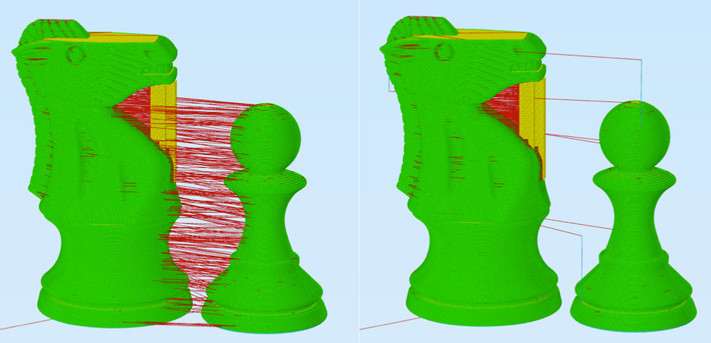
\includegraphics[width=0.5\textwidth,cfbox=azul_marcos 4pt 0pt]{FOTOS/SEQUENTIALPRINTING}
\caption*{Vergleichen des Drucks zwischen gleichzeitigem und sequentiellem Druckverfahren}
\end{figure}
Außerdem können diese kleinen Fäden zwischen den Stücken erscheinen, wenn mehrere Stücke zur gleichen Zeit gedruckt werden, da die Düse ständig von einem zum anderen Punkt springt.
\\\\
Wie wir zuvor bereits kommentiert hatten, kann dieser Effekt durch die Verwendung des Rückzugs reduziert werden, aber es ist sehr zu empfehlen, dass auch die unterschiedlichen Stücke sequenziell statt simultan gedruckt zu werden.
\\\\
Mit sequentiellem Druck meinen wir den Druck von einem Stück nach dem anderen, anstatt alle gleichzeitig nebeneinander zu drucken.
\\\\
Dies kann auf zwei verschiedene Arten erreicht werden:
\begin{itemize}
\item Die triviale Option ist nur ein Stück zu drucken und einmal abgeschlossen, wiederholen Sie den Druck so oft wie gewünscht.
\item Die zweite Alternative, weiter fortgeschritten und mit einigen Einschränkungen, ist die Laminierungsoption zu verwenden, dass einige Programme anstelle eines Drucks nach dem anderen anbieten. Die maximale Größe der Stücke, die durch dieses Verfahren gedruckt werden können, ist abhängig von der Abmessung der Düse und der Andordnung der unter Verwendung kommt durch die Abmessungen der Düse und die Anordnung der Exes des Druckers. Wir empfehlen dringend, dass Sie sich darüber informieren, wie die Optionen zu verwenden ist, um nicht die Gefahr einer Beschädigung des Druckers einzugehen. Sie können dies über die folgenden Links tun: 
\end{itemize}
\url{https://www.simplify3d.com/support/tutorials/multi-part-printing/}\\
\url{http://manual.slic3r.org/advanced/sequential-printing}\\
\url{https://ultimaker.com/en/community/3843-force-cura-to-print-objects-separately}
	\subsection{Die erste Schicht}
Die erste Schicht ist die Grundlage für den Rest der Schichten und kann den Unterschied zwischen einem zufriedenstellenden Druck und einem gescheiterten Druck darstellen.
\\\\
Beim Drucken mit FlexiSMART muss man besonderes ein Auge auf die erste Schicht haben, da ein Drucker, der korrekt auf PLA oder ABS nivelliert ist, dies eventuell nicht ist um mit FlexiSMART zu drucken.
\\\\
Um zu wissen, ob der Drucker richtig nivelliert ist, müssen Sie aufmerksam beobachten, wie die Maschine die erste Schicht erzeugt.
\\\\
Wenn die erste Schicht durchscheinend erscheint, bedeutet dies, dass die Düse zu nahe an der Plattform ist und es wird notwendig sein, sie einigen Mikrometer zu trennen.
\\\\
Wenn die erste Schicht sich hingegen abzulösen scheint oder sich immer wieder Lücken ohne Plastik zeigen, ist es erforderlich die Düse ein paar Mikrometer näher an die Plattform zu bringen.
\begin{figure}[H]
    \centering
    \begin{subfigure}[b]{0.3\textwidth}
        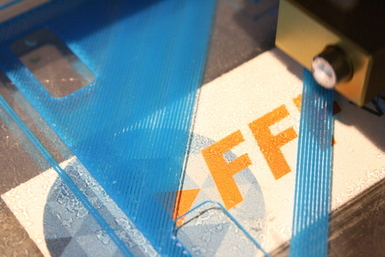
\includegraphics[width=\textwidth,cfbox=azul_marcos 3pt 0pt]{FOTOS/HOTENDALTO}
	\caption*{Nozzle too far}
    \end{subfigure}
    ~ %add desired spacing between images, e. g. ~, \quad, \qquad, \hfill etc. 
      %(or a blank line to force the subfigure onto a new line)
    \begin{subfigure}[b]{0.3\textwidth}
        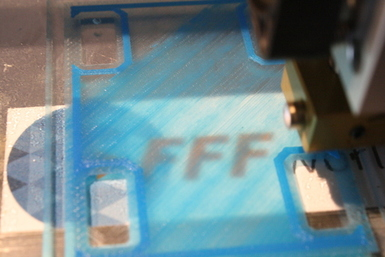
\includegraphics[width=\textwidth,cfbox=azul_marcos 3pt 0pt]{FOTOS/HOTENDBAJO}
	\caption*{Nozzle too close}
    \end{subfigure}
    ~ %add desired spacing between images, e. g. ~, \quad, \qquad, \hfill etc. 
    %(or a blank line to force the subfigure onto a new line)
    \begin{subfigure}[b]{0.3\textwidth}
        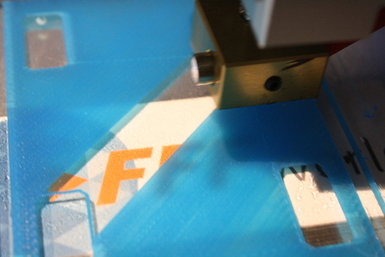
\includegraphics[width=\textwidth,cfbox=azul_marcos 3pt 0pt]{FOTOS/HOTENDPERFECTO}
	\caption*{Nozzle well leveled}
    \end{subfigure}
\end{figure}
Diese Anpassung kann per Software vorgenommen werden mittels einer Anpassung des z-offset in dem Laminierprogramm oder durch Regulieren der Ebnungsmechanismus der Druckplattform.
	\subsection{Beschichtungshinweise}
		\subsubsection{Die Höhe der Schicht}
Die Höhe der Schicht bestimmt die Qualität des Stückes und die Zeit des Druckens.
\\\\
Bei der Verwendung einer Düse von 0,4 mm haben wir gezeigt, dass die optimale Höhe der Schicht 0,2 mm ist. Mit dieser Schichthöhe werden Sie stark miteinander verbundene Schichten und einer ausgezeichneten Oberflächenqualität erhalten.
		\subsubsection{Die oberen Schichten und der Perimeter}
Die Top Layers und Perimeter sind das laterale und überlegene Umhüllen des Druckstückes. Die ausreichende Anzahl davon werden vom Infill abhängen und der Verwendung des Stückes.
\\\\
Mit einem hohen Infill können Sie die Top-Layer-Anzahl auf 3 reduzieren, da die Füllung des Stückes eine gute Basis gibt um darauf zu stehen. Mittlere oder niedrige Werte bei Infill zu verwenden wird empfohlen um die Anzahl der Top-Layer auf 5 anzuheben und um sicherzustellen, dass die Oberseite des Stücks vollständig abgedichtet ist.
\\\\
Wenn das Stück womöglich unter Verformungen leidet, ist es empfehlenswert die Anzahl der Shells oder horizontalen Perimeter zu steigern. Eine erhöhte Anzahl der horizontalen Perimeter wird eine Viertelung der Wände des Stückes vermeiden wenn auf sie Druck oder Zug ausgeübt wird.
\\\\
Diese Empfehlungen sind gültig, wenn Sie eine Düse von 0,4 mm und eine Schichthöhe von 0,2 mm verwenden. Wenn die Größe der Düse oder der Schicht variiert, ändern sich auch Anzahl der Perimeter und optimalen Top-Layer.
\\\\
Wir laden Sie ein Ihre eigenen Tests durchzuführen und die Ergebnisse mit uns zu teilen.
		\subsubsection{Einfluss der Infill-Flexibilität}
Die Menge und die Gestaltung der Füllung hat einen großen Einfluß auf den Grad der Flexibilität des Stücks beim Druck mit FlexiSMART.
\\\\
Ein Stück mit Infill nahe 100\% wird sich wie ein Gummiblock verhalten und kann eine gute Wahl für Stücke wie Silent-Block oder Spacern sein.
\\\\
Unter Verwendung einer Füllung aus 15\% werden Sie weiche Stücke erhalten, die gestaucht und verformt werden könnte.
\\\\
Das Infill-Muster wirkt sich auch auf die Flexibilität und eine geradlinige Füllung verhält sich nicht gleich einer Honeycomb-Füllung. Wir laden Sie ein Ihre eigenen Tests zu machen und die Füllung zu wählen, die am besten zu Ihrem Projekt passt.
	\subsection{Nutzung einer größeren Düse}
Der größere Teil der Drucker verwenden als Serie eine Düse von 0,4 mm, einer Düsengröße, die ein gutes Geschwindigkeit/Auflösungs-Verhältnis leifert. FlexiSMART ist perfekt für diese Art von Düse geeignet, jedoch ist es zweckmäßig einige Präzisierungen zu machen.
\\\\
Die Größe der Düse begrenzt die Menge an Material, das pro Zeiteinheit extrudiert werden kann. Durch die Verwendung von steifen Filamenten ist dieser Grenzwert höher, da die Geschwindigkeit erhöht werden kann und das Filament selbst den erforderlichen, zusätzlichen Druck für das Material beim Austritt aus der Düse unterstützt. Bei FlexiSMART werden die Filamente jedoch zusammengedrückt, wenn dieser Druck zu hoch ist und im allgemeinen muß bei niedrigeren Geschwindigkeiten gedruckt werden.
\\\\
Wenn Sie also FlexiSMART bei hohen Geschwindigkeiten extrudieren wollen, ist es empfehlenswert, dass Sie eine Düse verwenden ab der Größe von 0,6 mm. Mit einer dieser Düsen kann man viel schneller und mit überlegener Schichthöhe drucken, was etwas Auflösung kostet.
\section{Würden Sie unser Projekt gerne unterstützen?}
Alle Mitglieder von FFF World lieben den 3D-Druck und die Maker-Gemeinde. Wir sind glücklich in der Lage zu sein an Projekten zu arbeiten, bei denen wir unsere ehrliche Leidenschaft liefern können. In der Zukunft hoffen wir in der Lage zu sein mehr Materialien, mehr Farben und mehr Formate zu entwickeln.
\\\\
Daher ist es eine der besten Aktionen um uns zu helfen, sofern Sie es wollen und mit unserern Filamenten zufrieden sind, uns auf Amazon 5 Sterne zu geben.
\begin{figure}[H]
\centering

\includegraphics[width=0.5\textwidth,cfbox=azul_marcos 1pt 0pt]{FOTOS/AMAZON_FIVE_STARS}
\caption*{Vielen Dank!}
\end{figure}
\subsection{Andere Materialien mit fantastischen Charakteristika auf Amazon}
\begin{description}
\item[FlexiSMART Tech:] Entwickelt, um die Abnutzung und den Verschleiß von technischen Drücken zu widerstehen.
\item[ABS Tech:] Minimierter Warping-Effekt. Hohe Leistung bei technischen Anwendungen.
\item[PETG Tech:] Maximale mechanische Beständigkeit. Beständig beim Kontakt mit Wasser und UV-Strahlen. Geegnet für die Nahrungsbenutzung.
\item[FilaMETAL:] PLA mit nichtscheuernder, metallischer Ladung, die Ihren Skulpturen ein spektakuläres mechanisches Finish gibt.
\item[PC Tech:] Polycarbonate mit einer hohen Temperaturbeständigkeit und hervorragenden metallischen Eigenschaften.
\item[Nylon Tech:] Druckbar bei geringen Temperaturen. Widerstand gegen physische Krafteinwirkung mit einem gewissen Grad an Flexibilität.
\item[PVA Tech:] Löslich in Wasser, Filament angegeben für die Verwendung als Trägermaterial. Ausgezeichnet mit PLA kompatibel.
\item[HIPS Tech:] Löslich in Limonen Filament angegeben für die Verwendung als Trägermaterial. Gute mechanische Beständigkeit und eine ausgezeichnete Kompatibilität mit ABS.
\end{description}
%\section{Bibliografía}
%Esta guía no habría sido posible sin el conocimiento libre generado por la comunidad RepRap. Para la elaboración de esta guía se han %utilizado imágenes y contenido extraidos de los siguientes sitios web.
%\\\\
%\url{http://www.gyrobot.co.uk/blog/how-to-3d-print-with-flexible-filaments}\\
%\url{http://www.thingiverse.com/thing:1496895}\\
%\url{http://www.thingiverse.com/thing:247024}\\
%\url{http://www.thingiverse.com/thing:16319}\\
%\url{http://www.thingiverse.com/thing:779011}\\
%\url{http://www.thingiverse.com/thing:1102900}\\
%\url{http://www.thingiverse.com/thing:147705}\\
%\url{http://www.thingiverse.com/thing:222667}\\
%\url{http://www.thingiverse.com/thing:512338}\\
%\url{https://all3dp.com/common-3d-printing-problems-and-their-solutions/}\\
%\url{https://www.simplify3d.com/support/}\\
%\url{http://www.thingiverse.com/thing:508896}\\
%\url{http://www.thingiverse.com/thing:1187344}

\includepdf{PDF/DE_CONTRAPORTADA.pdf}
\end{document}
